En este apartado se presentan los diagramas de Gantt que inicialmente se plantearon para el proyecto.

\begin{figure}[H]
    \centering
    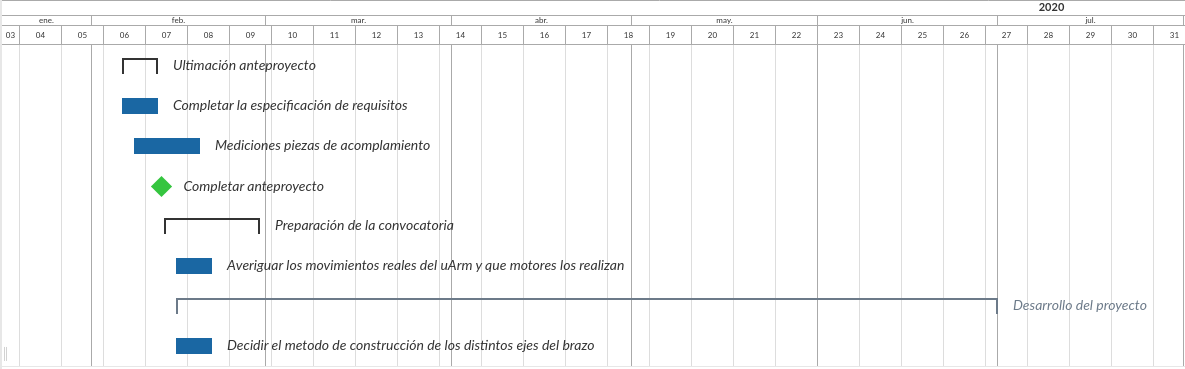
\includegraphics[width=\linewidth]{pictures/DiagramaGanttGeneral.png}
    \caption{Diagrama de Gantt general.}
    \label{fig:gantt_general}
\end{figure}

En el diagrama \ref{fig:gantt_general} se observa la planificación inicial del proyecto el cual tenía como fecha prevista de finalización el 30 de junio.

Se pueden observar que, a nivel general, la planificación constaba de tres partes:

\begin{itemize}
    \item El anteproyecto.
    \item La preparación para la convocatoria de soporte para el desarrollo de proyectos \ac{HW}.
    \item El desarrollo efectivo del proyecto.
\end{itemize}

El anteproyecto se desglosaba en las siguientes partes (figura \ref{fig:gantt_anteproyecto}):

\begin{figure}[H]
    \centering
    \includegraphics[width=\linewidth]{pictures/UltimaciónAnteproyecto.png}
    \caption{Diagrama de Gantt del anteproyecto.}
    \label{fig:gantt_anteproyecto}
\end{figure}

Para realizar el anteproyecto el equipo de desarrollo tuvo que investigar posibles materiales con los que podría ser construido el brazo, además de los acoplamientos mecánicos entre las distintas piezas. Esto ultimo era de especial importancia ya que escapaba al ámbito de conocimiento de los integrantes del equipo.

Por otro lado, se tenia que obtener una relación entre la masa que levantaría el brazo y la fuerza que han de ejercer los motores. Esto era de interés ya que se necesitaba elegir unos motores que fuesen capaces de, al menos, mover la estructura del brazo sin carga adicional. Por otro lado, y debido a que el proyecto fue propuesto para una ayuda económica para trabajos de fin de grado, era necesario una tabla detalla de presupuestos, y conocer el modelo de los motores a comprar y del microcontrolador a utilizar sería obligatorio a la hora de hacer dicha tabla.

mientras que en la figura \ref{fig:gantt_convocatoria} se muestran las distintas
labores que se realizaron para cumplimentar el documento requerido:

\begin{figure}[H]
    \centering
    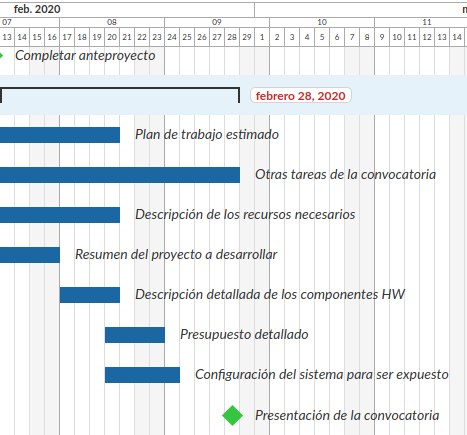
\includegraphics[width=1\linewidth]{pictures/PreparacionConvocatoria.png}
    \caption{Diagrama de Gantt de la preparación de la convocatoria}
    \label{fig:gantt_convocatoria}
\end{figure}

Para poder completar el documento que se requería presentar para beneficiar de la ayuda económica, el equipo de desarrollo describió un plan de trabajo estimado y empleando la tabla de presupuestos del anteproyecto hizo constar la necesidad de cada uno de los elementos que aparecían en esta.

Por otro lado, hizo una breve descripción del proyecto y dejo clara la relevancia de la parte hardware dentro de este. Finalmente, detalló la configuración que debería tener el sistema para poder hacer una demostración en caso de ser este expuesto.

Por su parte, la planificación técnica del proyecto se desglosa en el diagrama
\ref{fig:gantt_proyecto}:

\begin{figure}[H]
    \centering
    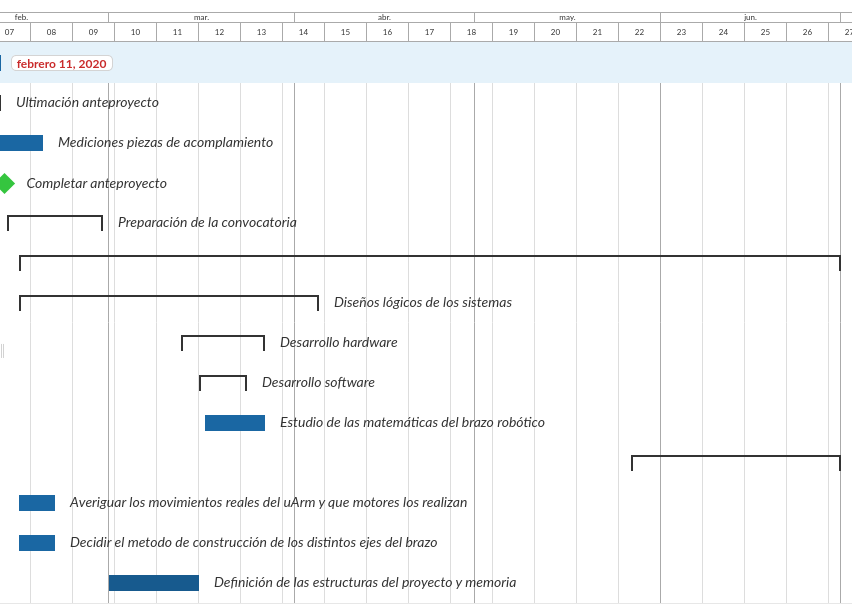
\includegraphics[width=1\linewidth]{pictures/DesarrolloProyecto.png}
    \caption{Diagrama de Gantt del desarrollo del proyecto}
    \label{fig:gantt_proyecto}
\end{figure}

En la planificación que el equipo había propuesto para el desarrollo del proyecto, se observa una división del software y del hardware en periodos de desarrollo individuales, y concurrentes entre si y con respecto al estudio del fundamento matemático del proyecto.

Por otro lado era necesario realizar un estudio de la manera en la que el movimiento conjunto de dos o más motores afectaba al movimiento del \textit{end--efector}. En relación al estudio de los acoplamientos mecánicos del brazo, el equipo de desarrollo debía decidir el método de construcción de los distintos ejes del brazo.

Finalmente se definiría la estructura del proyecto y la memoria ya que era intención del equipo de desarrollo realizar la documentación del proyecto en paralelo al desarrollo técnico de este.

La planificación temporal del proyecto se desglosa en múltiples apartados que no son
representados en las imágenes anteriores, pero se deja un enlace por si se quieren
consultar así como el detalle de cada una de las tareas propuestas:

\begin{center}
    \url{https://s.javinator9889.com/pArm-gantt} \qquad \qrcode{https://s.javinator9889.com/pArm-gantt}
\end{center}

Además, el diagrama al completo se encuentra también en el anexo \ref{anex:gantt}.
